\chapter{\ifenglish Background Knowledge and Theory\else ทฤษฎีที่เกี่ยวข้อง\fi}

\section{ด้านโครงสร้างเว็บ}
\subsection{MVC (Model-View-Controller)}
    เป็นรูปแบบในการออกแบบซอฟต์แวร์ที่ใช้กันทั่วไปในการปรับใช้หน้าแสดงผล ข้อมูล แลการควบคุม เน้นการแยกระหว่างตรรกะทางธุรกิจของซอฟต์แวร์และการแสดงหน้าแสดงผล "การแยกส่วน" นี้ทำให้มีการแบ่งงานที่ดีและแก้ไขได้ง่ายขึ้น หรือเรียกได้ว่าเป็น Design pattern ที่ช่วยเพื่อช่วยสร้าง framework ให้กับ application โดยแบ่งเป็น Model, View และ Controller

\paragraph*{โมเดล(Model)}
    ส่วนของซอฟต์แวร์ที่ใช้ในการแปลการทำงานของระบบ ไปสู่สิ่งที่ระบบซอฟต์แวร์ได้ถูกออกแบบเอาไว้ ตรรกะเนื้อหาใช้เพื่อให้ความหมายแก่ข้อมูลดิบ (ยกตัวอย่างเช่น การคำนวณว่าวันนี้เป็นวันเกิดของผู้ใช้หรือไม่, หรือจำนวนเงินรวม ภาษี และค่าส่งสินค้า ในตะกร้าสินค้า) เมื่อโมเดลมีการเปลี่ยนแปลง จะมีการส่งคำเตือนให้แก่ วิว ที่เกี่ยวข้องเพื่อปรับค่า
ระบบซอฟต์แวร์หลายระบบใช้การเก็บข้อมูลถาวร เช่น ฐานข้อมูล เพื่อเก็บข้อมูลเหล่านี้ MVC ไม่ได้กำหนดถึงระดับการเข้าถึงข้อมูล เพราะเป็นที่เข้าใจกันว่าส่วนนี้จะอยู่ภายใต้ หรือถูกครอบคลุมด้วยโมเดล โมเดลไม่ได้เป็นเพียงอ็อบเจกต์ที่ใช้เข้าถึงข้อมูล แต่ในระบบซอฟต์แวร์เล็กๆ ซึ่งมีความซับซ้อนน้อยจะไม่เห็นความแตกต่างมากนัก 

\paragraph*{วิว(View)}
    แสดงผลค่าในโมเดลในรูปแบบที่เหมาะสมต่อการปฏิสัมพันธ์กับผู้ใช้ ในแต่ละโมเดลสามารถมีวิวได้หลายแบบ เพื่อใช้ในจุดประสงค์ที่ต่างกัน 

\paragraph*{คอนโทรลเลอร์ (Controller)}
    รับข้อมูลจากผู้ใช้เข้ามา แล้วดำเนินการตอบสนองต่อข้อมูลนั้น โดยเรียกใช้ logic ต่างๆจากอ็อบเจกต์ในโมเดล และส่งข้อมูลผลลัพย์นั้นกลับไปยังส่วนแสดงผล เพื่อตอบกลับไปยังผู้ใช้ได้อย่างถูกต้อง 

\newpage
\begin{figure}[h]
        \centering
        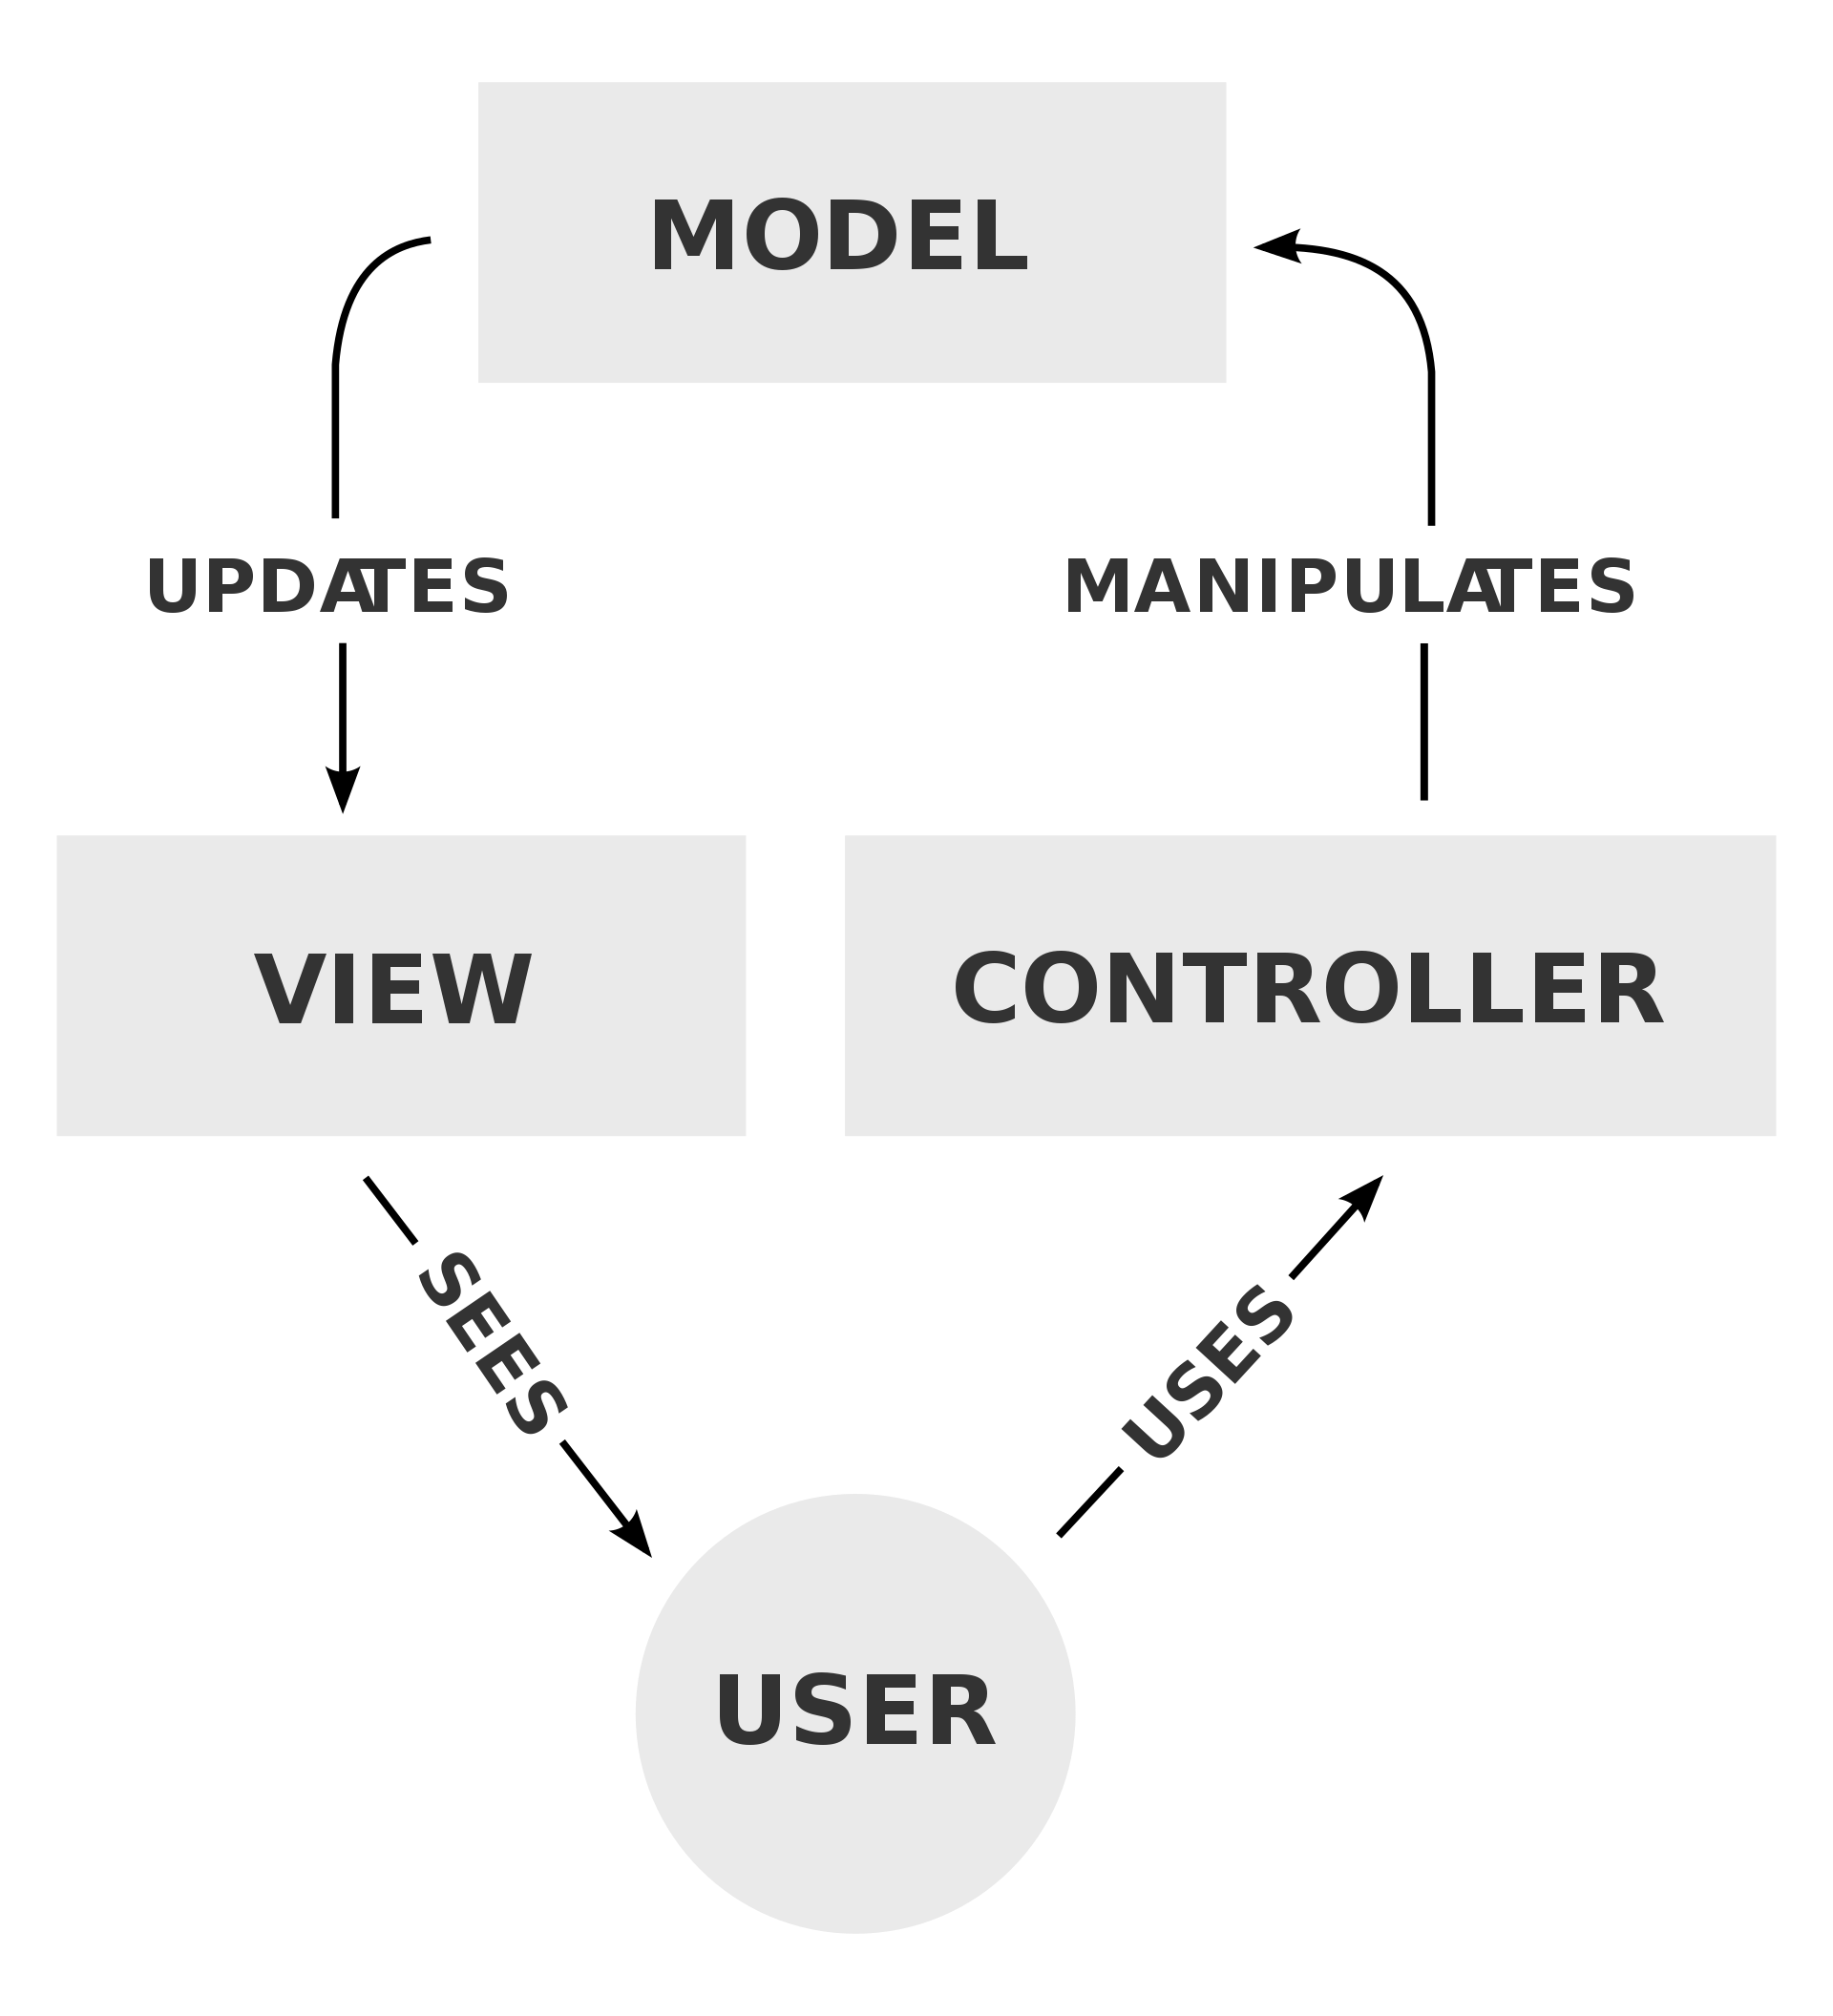
\includegraphics[width= 0.5\textwidth]{mvc.png}
        \caption{MVC}
        \label{fig: mvc (Model-View-Controller)}
\end{figure}
โดยเรานำมาใช้โดยแบ่งส่วนของ MVC ให้เป็น 3 ส่วนดังนี้
Model
จัดการฐานข้อมูลและ business logic ในโปรเจคนี้จะเป็นการวางวิธีการจัดเก็บข้อมูลใน database
View
ส่วนของ layout และการแสดงผล ( รวมถึง user interface และ user experience ) ในโปรเจคนี้จะเป็นหน้าการแสดงผลทั้งหมด
Controller
Route ของการทำงานต่างๆ ที่สามารถเข้าไปแก้ไขหรือทำการอัพเดต Model

% \CIreply{need citation to each of these technologies}
\subsection{RESTful api}
\par เป็นอินเทอร์เฟซที่ระบบคอมพิวเตอร์สองระบบใช้เพื่อแลกเปลี่ยนข้อมูลผ่านอินเทอร์เน็ตได้อย่างปลอดภัย แอปพลิเคชั่นทางธุรกิจส่วนใหญ่ต้องสื่อสารกับแอปพลิเคชันภายในอื่นๆ และของบุคคลที่สามเพื่อทำงานต่างๆ ตัวอย่างเช่น หากต้องการสร้างสลิปเงินเดือน ระบบบัญชีภายในของคุณต้องแบ่งปันข้อมูลกับระบบธนาคารของลูกค้าเพื่อออกใบแจ้งหนี้และสื่อสารกับแอปพลิเคชันบันทึกเวลาปฏิบัติงานภายในโดยอัตโนมัติ RESTful API ให้การสนับสนุนการแลกเปลี่ยนข้อมูลนี้เพราะเป็นระบบที่มีมาตรฐานการสื่อสารระหว่างซอฟต์แวร์ที่ปลอดภัย เสถียร และมีประสิทธิภาพ และสามารถนำมาใช้กับโมเดลแบบ MVC ได้ด้วยโดยใช้ RESTful API โดยจะมีคำสั่งที่ทำจาก Controller เพื่อส่งไปหา Model และมีคำสั่งที่ View จะรับข้อมูลมาจาก Model

\paragraph*{Get}
ทางฝั่งของ Client ใช้ GET เพื่อเข้าถึงทรัพยากรที่อยู่ที่ URL ที่ระบุบนเซิร์ฟเวอร์ ซึ่งสามารถแคชคำขอ GET และส่งพารามิเตอร์ในคำขอ RESTful API เพื่อสั่งให้เซิร์ฟเวอร์กรองข้อมูลก่อนส่ง

\paragraph*{Post}
ทางฝั่งของ Client ใช้ POST เพื่อส่งข้อมูลไปยังเซิร์ฟเวอร์ ซึ่งรวมถึงการแทนข้อมูลพร้อมกับคำขอ การส่งคำขอ POST เดียวกันหลายครั้งมีผลข้างเคียงเหมือนกับการสร้างทรัพยากรเดียวกันหลายครั้ง

\paragraph*{Put}
ทางฝั่งของ Client ใช้ PUT เพื่ออัปเดตทรัพยากรที่มีอยู่บนเซิร์ฟเวอร์ การส่งคำขอ PUT เดียวกันหลายครั้งในบริการเว็บ RESTful จะให้ผลลัพธ์เหมือนกัน ซึ่งแตกต่างจาก POST

\paragraph*{Delete}
ทางฝั่งของ Client ใช้คำขอ DELETE เพื่อลบทรัพยากรออก โดยคำขอ DELETE สามารถเปลี่ยนสถานะเซิร์ฟเวอร์ได้ อย่างไรก็ตาม หากผู้ใช้ไม่มีการรับรองความถูกต้องที่เหมาะสม คำขอก็จะล้มเหลว

โดยการต่อ api นั้นยังมีรหัสที่บ่งบอกถึงสถานะการติดต่อทั่วไป เช่น
\begin{itemize}
    \item 200: การตอบสนองเพื่อระบุถึงความสำเร็จทั่วไป
    \item 201: การตอบสนองเพื่อระบุถึงความสำเร็จของวิธีการ POST
    \item 400: คำขอที่ไม่ถูกต้องที่เซิร์ฟเวอร์ไม่สามารถประมวลผลได้
    \item 404: ไม่พบทรัพยากร
    \item 500: ช่องทางการติดต่อไม่ถูกต้อง
\end{itemize}

\section{Technology}
ในส่วนต่อไปนี้จะเป็นการอธิบายในเรื่องของเทคโนโลยีที่ใช้ในการพัฒนาเว็บแอพพลิเคชัน

\subsection{HTML}
HTML~ \cite{HTML} ย่อมาจาก HyperText Markup Language เป็น ภาษาคอมพิวเตอร์ท่ีใช้สร้างหน้าเว็บในรูปแบบของไฟล์ HTML (คือไฟล์ที่มีนามสกุลเป็น .htm หรือ .html) ซึ่งมีเว็บเบราว์เซอร์เป็นโปรแกรมที่ใช้แปลงไฟล์ HTML เพื่อ แสดงผลในรูปของหน้าเว็บ
ไฟล์ HTML บันทึกในรูปของไฟล์เอกสาร (text file) ที่สามารถถูกสร้างจากโปรแกรมสร้างไฟล์ ข้อความ เช่น Notepad หรือ word processing ทั่วๆ ไป ซึ่งลักษณะของไฟล์ HTML ประกอบไปด้วยแท็กต่างๆ ที่เป็นคำสั่งของ HTML ซึ่งแท็กจะอยู่ภายในเครื่องหมาย < และ >

\subsection{CSS}
CSS~ \cite{CSS} ย่อมาจาก Cascading Style Sheet  มักเรียกโดยย่อว่า style sheet คือภาษาที่ใช้เป็นส่วนของการจัดรูปแบบการแสดงผลเอกสาร  HTML โดยที่ CSS กำหนดกฏเกณฑ์ในการระบุรูปแบบ (หรือ style) ของเนื้อหาในเอกสาร 
อันได้แก่ สีของข้อความ สีพื้นหลัง ประเภทตัวอักษร และการจัดวางข้อความ ซึ่งการกำหนดรูปแบบนี้ใช้หลักการของการแยกเนื้อหาเอกสาร HTML ออกจากคำสั่งที่ใช้ในการจัดรูปแบบการแสดงผล กำหนดให้รูปแบบของการแสดงผลเอกสาร 
ไม่ขึ้นอยู่กับเนื้อหาของเอกสาร เพื่อให้ง่ายต่อการจัดรูปแบบการแสดงผลลัพธ์ของเอกสาร HTML

\subsection{JavaScript}
JavaScript~ \cite{JavaScript} หรือย่อด้วย JS เป็นภาษาเขียนโปรแกรมที่ถูกพัฒนาและปฏิบัติตามข้อกำหนดมาตรฐานของ ECMAScript
ภาษา JavaScript นั้นเป็นภาษาระดับสูง คอมไพล์ในขณะที่โปรแกรมรัน (JIT) และเป็นภาษาเขียนโปรแกรมแบบหลายกระบวนทัศน์ เช่น การเขียนโปรแกรมเชิงขั้นตอน การเขียนโปรแกรมเชิงวัตถุ หรือการเขียนโปรแกรมแบบ functional 
ภาษา JavaScript มีไวยากรณ์ที่เหมือนกับภาษา C ใช้วงเล็บเพื่อกำหนดบล็อกของคำสั่ง นอกจากนี้ JavaScript ยังเป็นภาษาที่มีประเภทข้อมูลแบบไดนามิกส์ เป็นภาษาแบบ prototype-based และ first-class function
%
ถือว่าเป็นเทคโนโลยีหลักของการพัฒนาเว็บไซต์ มันทำให้หน้าเว็บสามารถตอบโต้กับผู้ใช้ได้โดยที่ไม่จำเป็นต้องรีเฟรชหน้าใหม่ (dynamic website) เว็บไซต์จำนวนมากใช้ภาษา JavaScript 
สำหรับควบคุมการทำงานที่ฝั่ง client-side นั่นทำให้เว็บเบราว์เซอร์ต่างๆ มี JavaScript engine ที่ใช้สำหรับประมวลผลสคริปของภาษา JavaScript ที่รันบนเว็บเบราว์เซอร์

\subsection{Node.js}
Node.js~ \cite{NodeJS} คือสภาพแวดล้อมการทำงานของภาษา JavaScript นอกเว็บเบราว์เซอร์ที่ทำงานด้วย V8 engine กล่าวคือ สามารถใช้ Node.js ในการพัตนาแอพพลิเคชันแบบ command line แอพพลิเคชัน desktop หรือแม้แต่เว็บเซิร์ฟเวอร์ได้ 
โดยที่ Node.js จะมี APIs ที่เราสามารถใช้สำหรับทำงานกับระบบปฏิบัติการ เช่น การรับค่าและการแสดงผล การอ่านเขียนไฟล์ และการทำงานกับเน็ตเวิร์ก เป็นต้น

\subsection{React.JS}
React~ \cite{ReactJS} เป็น JavaScript library ที่ใช้สำหรับสร้าง user interface ในฝั่งด้าน front-end ที่ให้เราสามารถเขียนโค้ดในการสร้าง UI ที่มีความซับซ้อนแบ่งเป็นส่วนเล็กๆ ออกจากกันได้ ซึ่งแต่ละส่วนสามารถแยกการทำงานออกจากกันได้อย่างอิสระ 
และทำให้สามารถนำชิ้นส่วน UI เหล่านั้นไปใช้ซ้ำได้อีก

\subsection{MySQL}
MySQL~ \cite{MySQL} MySQL ซึ่งเป็นระบบจัดการฐานข้อมูลเชิงสัมพันธ์แบบโอเพนซอร์ส (RDBMS) มีมาตั้งแต่ปี 1995 ถูกสร้างขึ้นโดย MySQL AB ซึ่งต่อมาได้กลายเป็น Oracle Corporation ซอฟต์แวร์ใช้ SQL เป็นภาษาข้อมูลพื้นฐานและจัดเก็บข้อมูลในตารางบนดิสก์ไดรฟ์ของเซิร์ฟเวอร์ ข้อมูลสามารถจัดเก็บได้อย่างอิสระภายในขอบเขตที่กำหนดหรือเชื่อมโยงกับสคีมาที่กำหนดวิธีการจัดโครงสร้าง

\subsection{JSON}
JSON~ \cite{1_JSON} ย่อมาจาก JavaScript Object Notation เป็นฟอร์แมตสำหรับแลกเปลี่ยนข้อมูลคอมพิวเตอร์
ฟอร์แมต JSON นั้นอยู่ในรูปข้อความธรรมดา (plain text) ที่ทั้งมนุษย์และโปรแกรมคอมพิวเตอร์สามารถอ่านเข้าใจได้ 
มีนามสกุลของไฟล์เป็น .json ปัจจุบัน JSON นิยมใช้ในเว็บแอปพลิเคชัน โดย JSON เป็นฟอร์แมตทางเลือกในการส่งข้อมูล นอกเหนือไปจาก XML ซึ่งนิยมใช้กันอยู่แต่เดิม 
สาเหตุที่ JSON เริ่มได้รับความนิยมเป็นเพราะกระชับและเข้าใจง่ายกว่า XML เนื่องจากไฟล์ XML มีหน้าตาเป็นการเก็บข้อมูลโดยเก็บไว้ใน tag
ที่จะต้องมี <tag> เปิดและ </tag> ปิด เหมือนกับ HTML ทำให้การเก็บข้อมูแต่ละตัวต้องใช้พื้นที่มากขึ้น

JSON~  \cite{2_JSON} นั้นใช้ในการเก็บข้อมูลโดยมีการรับและส่งไฟล์ด้วยภาษา JavaScript แต่ไม่ถูกมองว่าเป็นภาษาโปรแกรม กลับถูกมองว่าเป็นภาษาในการแลกเปลี่ยนข้อมูลมากกว่า 
ในปัจจุบันมีไลบรารีของภาษาโปรแกรมอื่นๆ ที่ใช้ประมวลผลข้อมูลในรูปแบบ JSON มากมาย

\subsection{Relational Database (RDBMS)}
เป็นฐานข้อมูล(Database)ประเภทหนึ่งที่จัดเก็บและให้การเข้าถึงจุดข้อมูลที่เกี่ยวข้องกัน ขึ้นอยู่กับแบบจำลองเชิงสัมพันธ์ (Relational Model) ซึ่งเป็นวิธีที่ง่ายและตรงไปตรงมาในการแสดงข้อมูลในตาราง ในฐานข้อมูลเชิงสัมพันธ์ แต่ละแถวในตารางเป็นข้อมูลที่มี ID เฉพาะที่เรียกว่าคีย์ คอลัมน์ของตารางมีแอตทริบิวต์ (attribute)ของข้อมูล และแต่ละระเบียนมักจะมีค่าสำหรับแต่ละแอตทริบิวต์ ทำให้ง่ายต่อการสร้างความสัมพันธ์ระหว่างจุดข้อมูลในแต่ละตาราง และในทุกตารางจะมีความความสัมพันธ์กัน


\section{ด้าน User Interface}

\subsection*{Design Thinking}

\subsection*{User-Centered Design Process}
เป็นหนึ่งในขั้นตอนที่สำคัญของการออกแบบ user experience การออกแบบนี้จะให้ความสำคัญและขึ้นอยู่กับความเข้าใจที่ชัดเจนของผู้ใช้งาน และสภาพแวดล้อมที่ได้รับการขับเคลื่อนและปรับแต่งโดยการประเมินที่เน้นผู้ใช้เป็นศูนย์กลาง และกล่าวถึงประสบการณ์ของผู้ใช้ทั้งหมด หมดทั้งกระบวนการนี้เป็น กระบวนการเกี่ยวข้องกับผู้ใช้ตลอดกระบวนการทั้งการออกแบบ การพัฒนาและการทำซ้ำของการออกแบบโปรแกรม


\section{\ifcpe%
ความรู้ตามหลักสูตรซึ่งถูกนำมาใช้หรือบูรณาการในโครงงาน
\else%
ISNE knowledge used, applied, or integrated in this project
\fi
}
\paragraph{261207 Basic CPE Lab}
นำความรู้ทางด้าน HTML, CSS, JavaScript และ React.JS รวมถึง Node.js 
ทั้งด้านของ front-end ที่แสดงผลผ่านเว็บไซต์ และ back-end ที่เชื่อมต่อกับฐานข้อมูล

\paragraph{261342 Database Systems}
การนำข้อมูลมาเก็บในรูปแบบตาราง การทำ UML และการออกแบบ ER diagrams ของเว็บแอพพลิเคชั่นที่จะทำ

\paragraph{261361 Software Engineering}
การใช้กระบวนการทางวิศวกรรมในการดูแลการผลิต ตั้งแต่การเริ่มเก็บความต้องการ การตั้งเป้าหมายของระบบ 
การออกแบบ กระบวนการพัฒนา การตรวจสอบ การประเมินผล และทดสอบระบบ

\paragraph{261102 Computer Programming}
การเขียน ทดสอบ และดูแลซอร์สโค้ดของโปรแกรมคอมพิวเตอร์ ซึ่งซอร์สโค้ดนั้นจะเขียนด้วยภาษาโปรแกรม 
ขั้นตอนการเขียนโปรแกรมต้องการความรู้ในหลายด้านด้วยกัน รวมถึงการนำ GitHub มาใช้ในการเขียนโปรแกรม

\section{\ifcpe%
ความรู้นอกหลักสูตรซึ่งถูกนำมาใช้หรือบูรณาการในโครงงาน
\else%
Extracurricular knowledge used, applied, or integrated in this project
\fi
}
\paragraph{User interface and user experience}
จะทำงานเกี่ยวกับการค้นคว้าหาข้อมูล ทำความเข้าใจถึงความต้องการของผู้ใช้งาน เพื่อให้ทราบถึงปัญหาของผู้ใช้งาน
ออกแบบสินค้าและบริการให้ตรงความต้องการผู้ใช้มากที่สุด ซึ่งหน้าที่หลัก ๆ ของ UX design คือ 
รวบรวมข้อมูลเกี่ยวกับผู้ใช้งาน รวมถึงทำการค้นคว้า ออกแบบ ทดสอบ และประเมินผลสิ่งต่าง ๆ 
ที่เกี่ยวข้องกับผู้ใช้งาน และทำการออกแบบต่าง ๆ เพื่อนำมาประยุกต์กับการออกแบบประสบการณ์ผู้ใช้
 เช่น design thinking, design sprint และ Lean UX
